\section{Gallery}
\label{sec:vis_gallery}
A picture is worth a thousand words. In this section we will show some screen shots from the visualization tool we have made. The DSMC visualizer can both render the state of the system while it integrates the system forward in time - a live visualization. This makes it easier to find interesting regions in the system, or is great as a show-off case.

\begin{figure}[htb]
\begin{center}
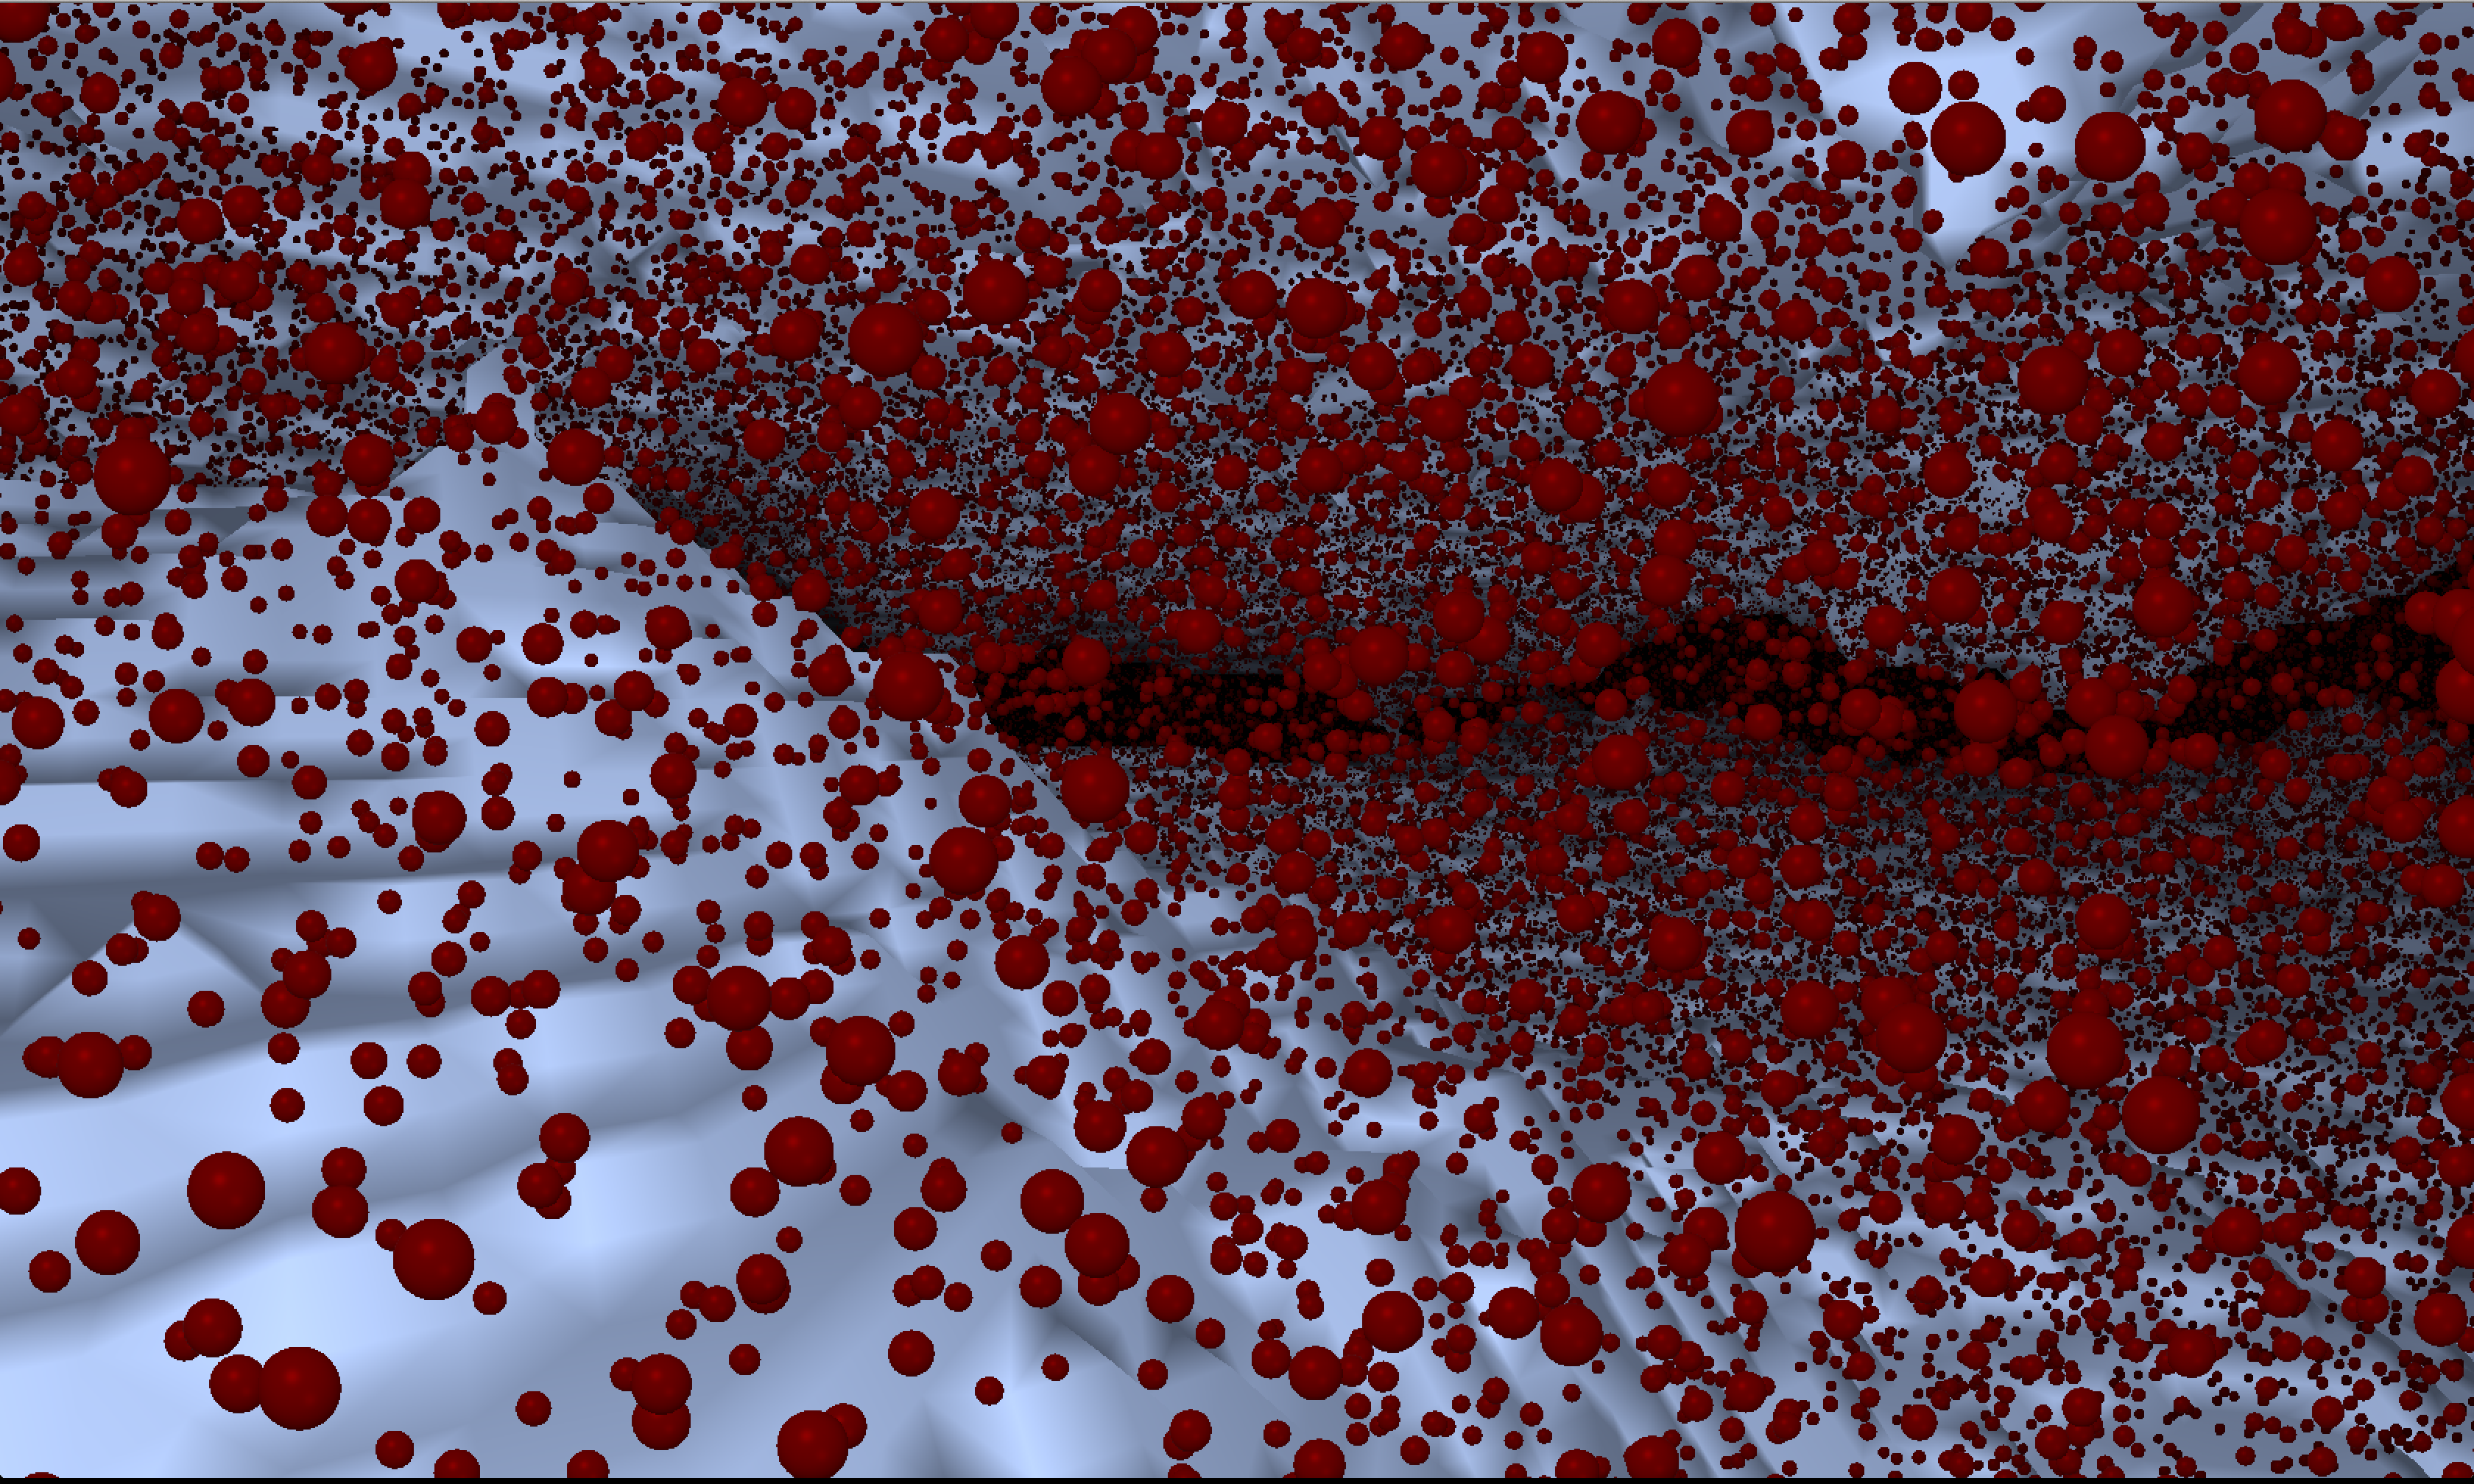
\includegraphics[width=\textwidth, trim=0cm 0cm 0cm 0cm, clip]{visualization/figures/marching_cubes_fracture.png}
\end{center}
\caption{Here we see a live simulation on a 2013 Macbook Pro. One million DSMC particles in a fracture created with the diamond-square algorithm (a thanks to Filip Sund who implemented this algorithm). We use billboards to render the particles and the marching cubes algorithm to create a smooth surface from the voxelized scalar field. With a good frame rate it is easy to study flow in any region of the system.}
\label{fig:vis_marching_cubes_2}
\end{figure}

\begin{figure}[htb]
\begin{center}
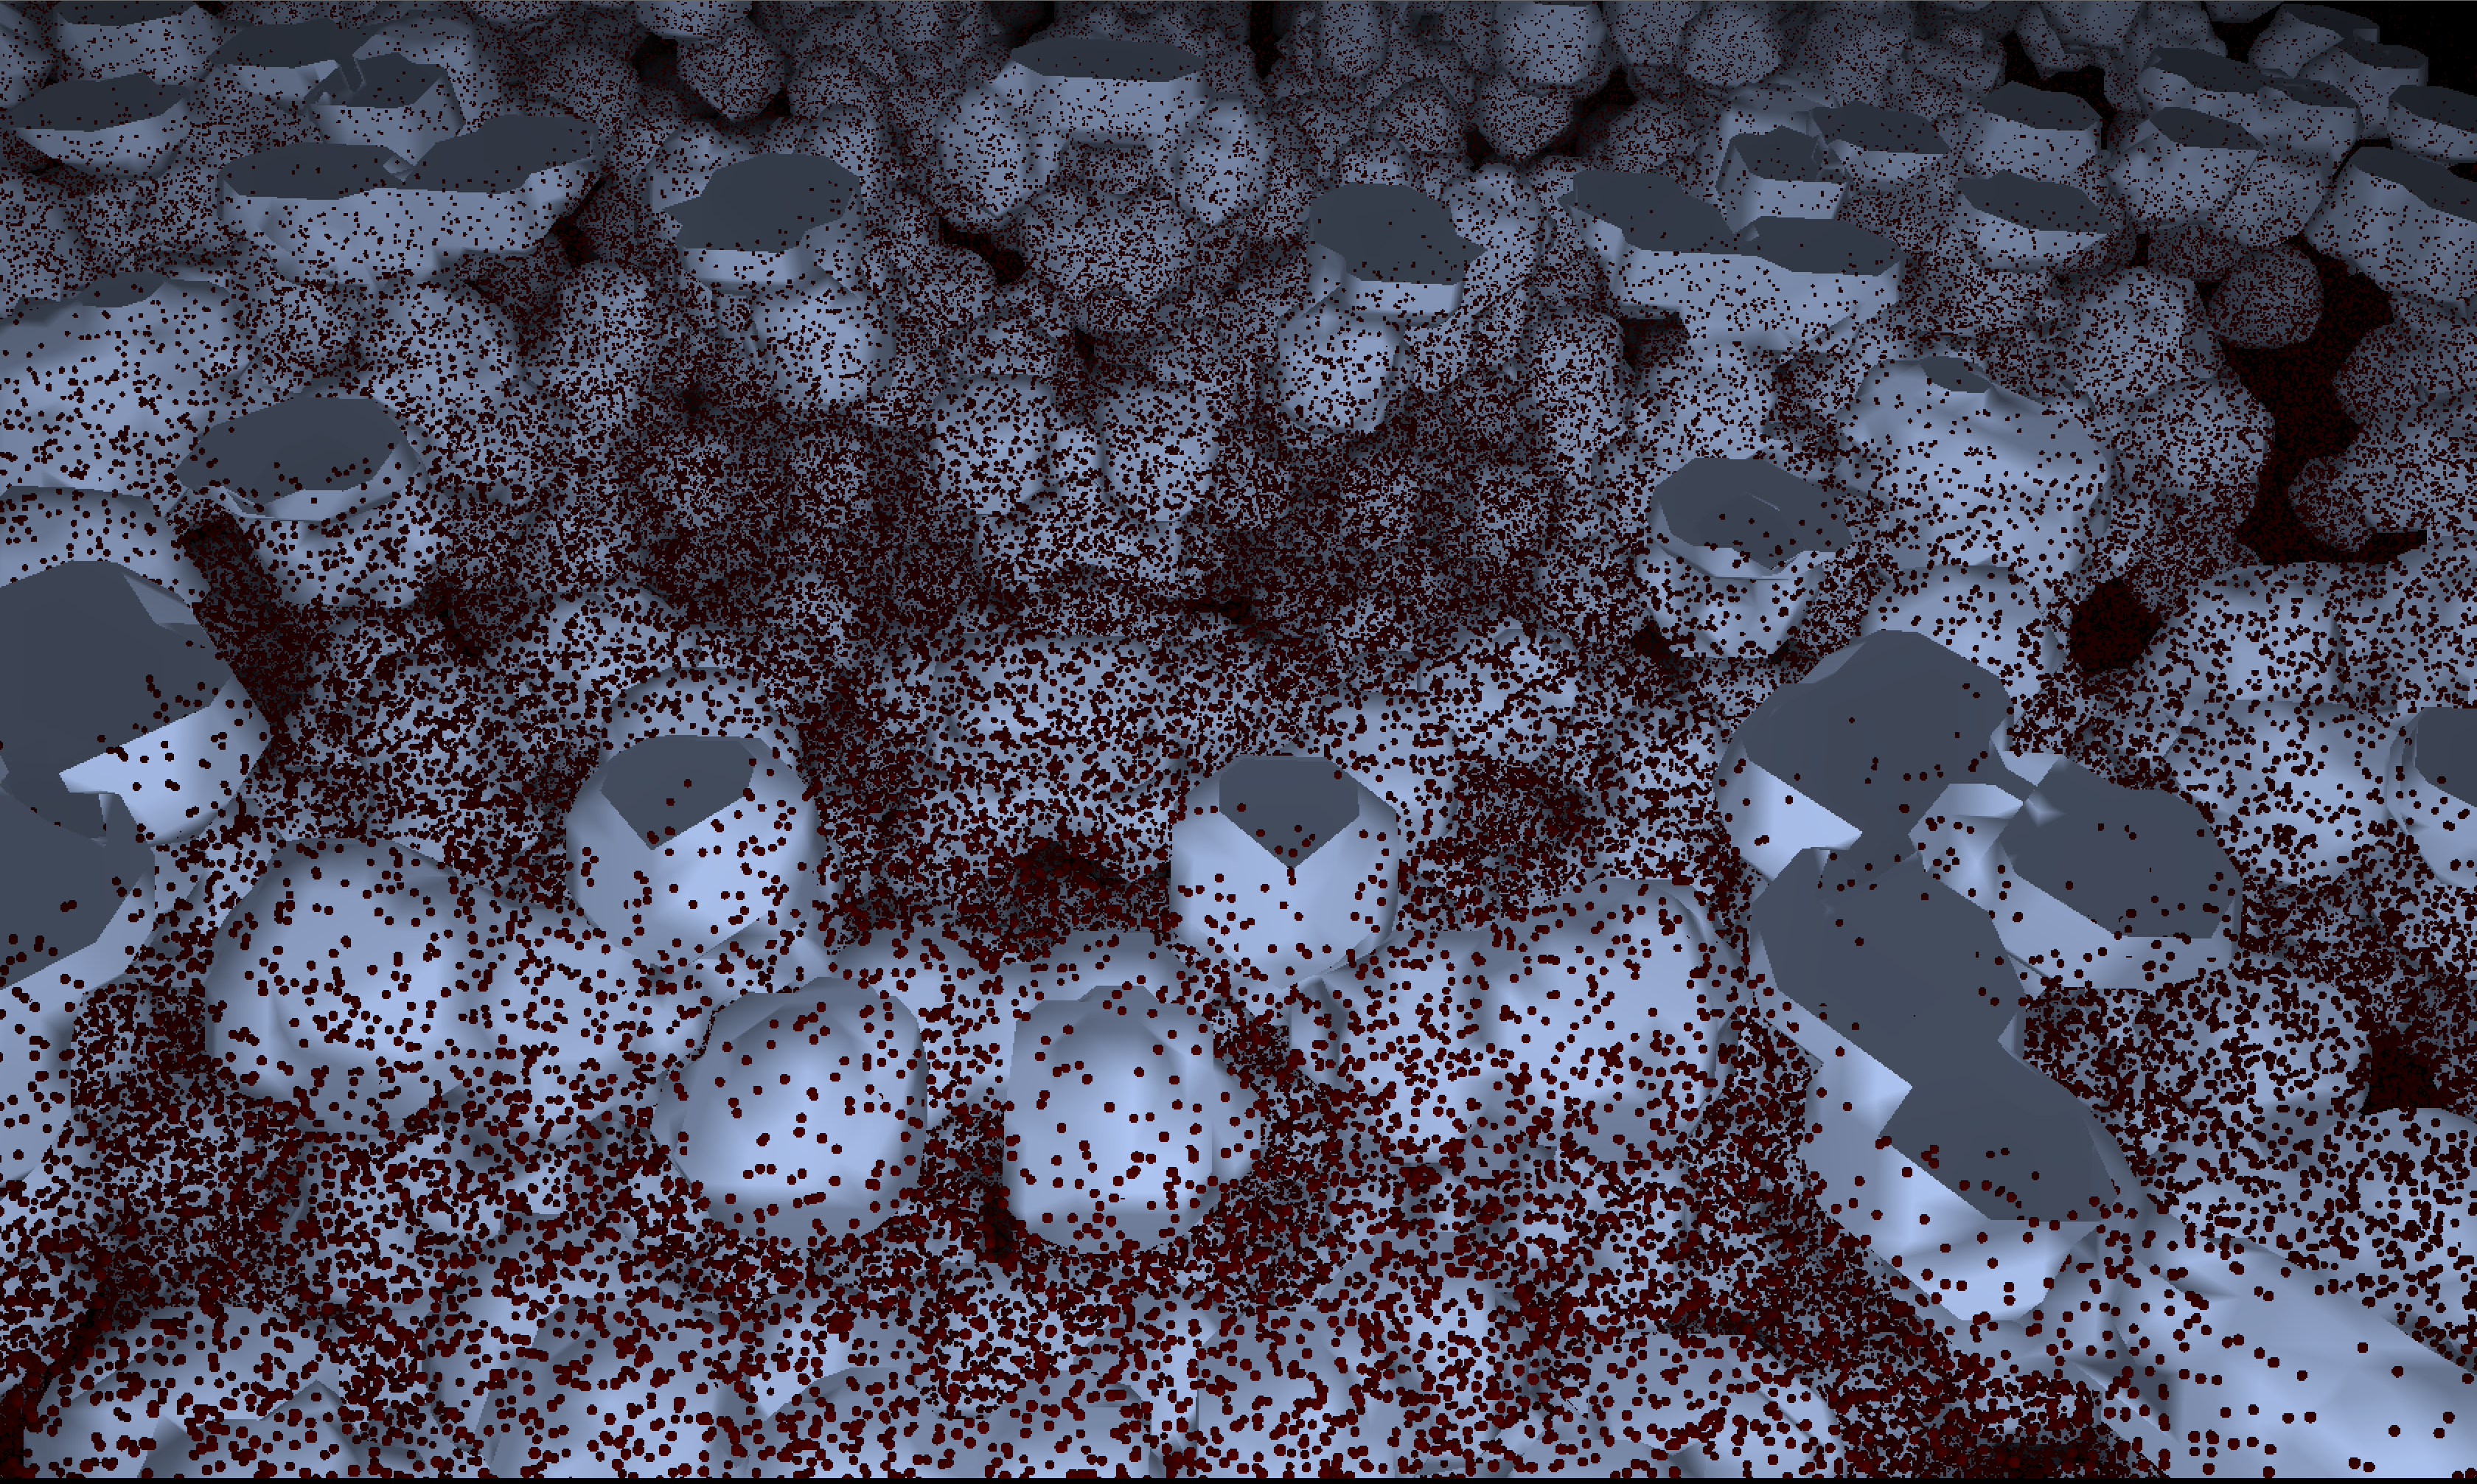
\includegraphics[width=\textwidth, trim=0cm 0cm 0cm 0cm, clip]{visualization/figures/marching_cubes_spheres_2.png}
\end{center}
\caption{This is a live simulation of four million DSMC particles in a system consisting of packed spheres using the same rendering technique as in figure \ref{fig:vis_marching_cubes_2}. The camera is placed outside the system where we clearly see some of the spheres being cut in half because of periodic boundary conditions. }
\label{fig:vis_marching_cubes_3}
\end{figure}

\begin{figure}[htb]
\begin{center}
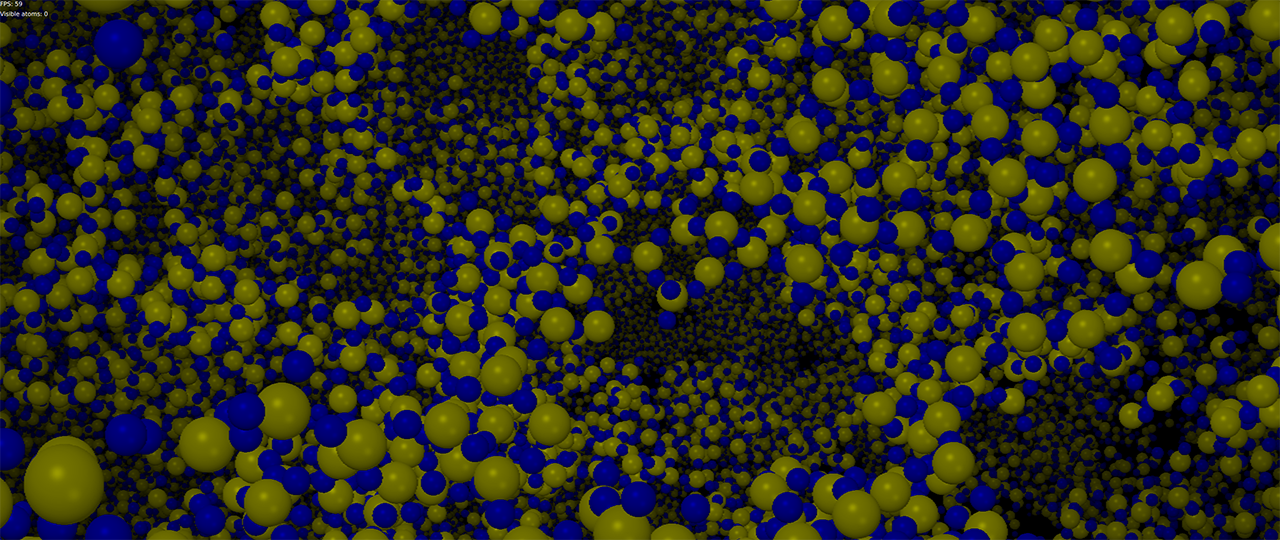
\includegraphics[width=\textwidth, trim=0cm 0cm 0cm 0cm, clip]{visualization/figures/md1.png}
\end{center}
\caption{Here we see a nanoporous silicate simulated with an MD code developed at the University of Southern California. The system was created by preparing the system in the $\beta$-cristobalite state. It was then heated to \unit{4500}{\kelvin}, stretched (increasing the system size) before it was cooled down, quenched, to \unit{300}{\kelvin} making this beautiful pore network. The pores were then filled with water. The total system consists of approximately 400,000 atoms, including water as shown in figure \ref{fig:vis_md3}.}
\label{fig:vis_md2}
\end{figure}

\begin{figure}[htb]
\begin{center}
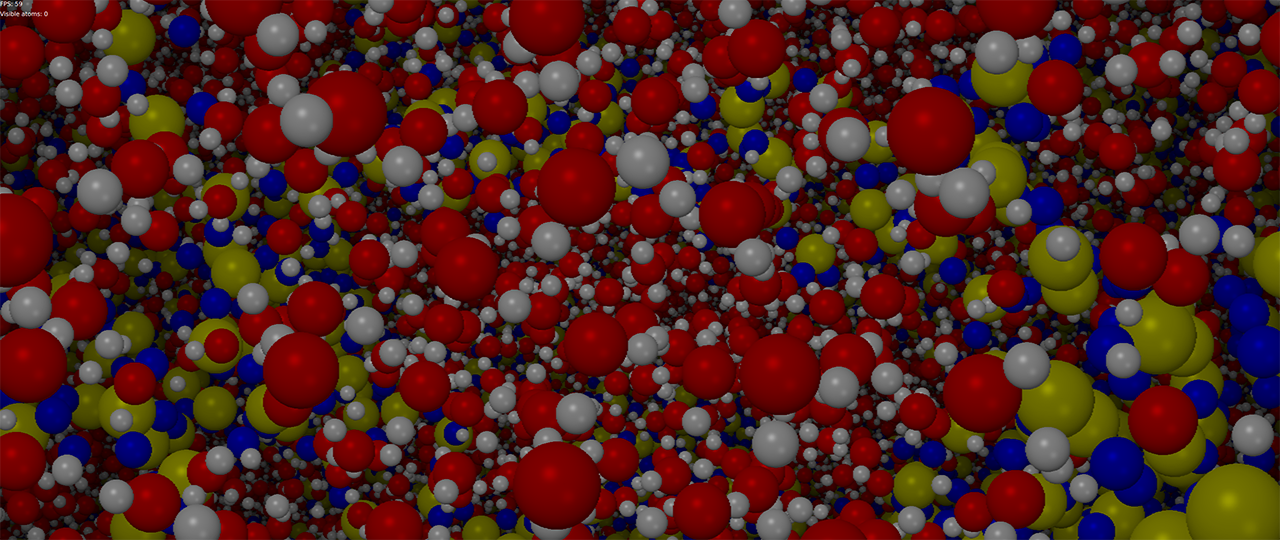
\includegraphics[width=\textwidth, trim=0cm 0cm 0cm 0cm, clip]{visualization/figures/md2.png}
\end{center}
\caption{This is the same system as in figure \ref{fig:vis_md2}, but with the water visible. We clearly see the water molecules form with one oxygen and two hydrogen atoms. With a non-static picture, with time evolution, we see the hydrogen atoms vibrate and even change which water molecule it is a part of. }
\label{fig:vis_md3}
\end{figure}

\begin{figure}[htb]
\begin{center}
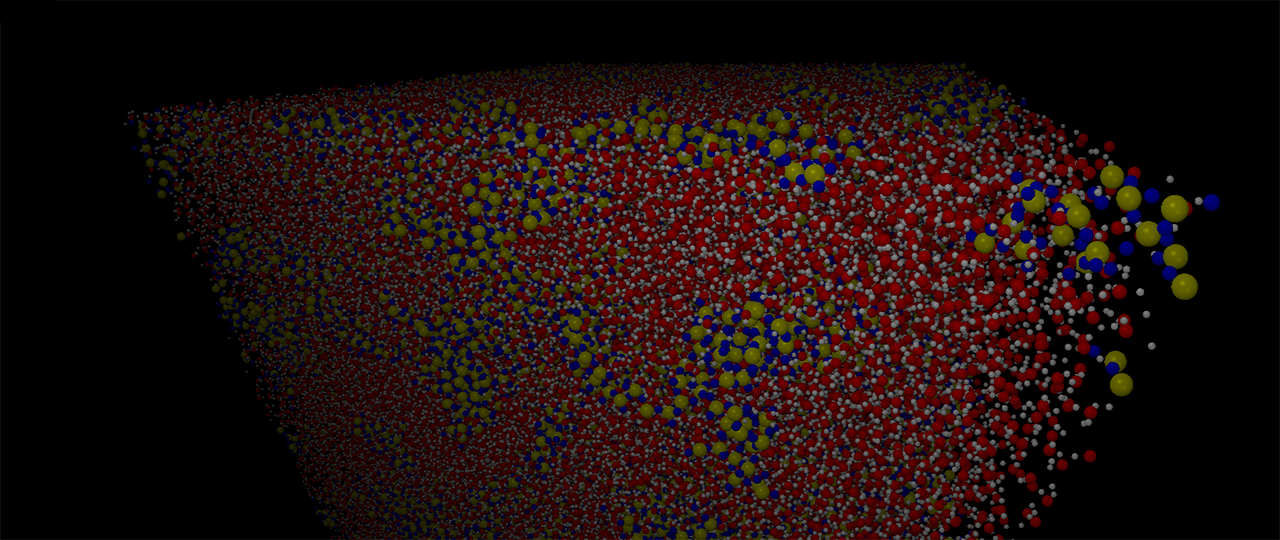
\includegraphics[width=\textwidth, trim=0cm 0cm 0cm 0cm, clip]{visualization/figures/md3.png}
\end{center}
\caption{Again the same system as in figures \ref{fig:vis_md2} and \ref{fig:vis_md3}, but with the camera outside the system. }
\label{fig:vis_md4}
\end{figure}